\achapter{15}{Subspaces}\label{chap:subspaces}


\vspace*{-17 pt}
\framebox{
\parbox{\dimexpr\linewidth-3\fboxsep-3\fboxrule}
{\begin{fqs}
\item What is a subspace of a topological space?
\item How do we define the subspace topology?
\item What are relatively open and closed sets?
\item To what kind of spaces is $\R$ with the standard topology homeomorphic?
\end{fqs}}}

\vspace*{13 pt}

\csection{Introduction}\label{sec_sub}

We have seen that a subset $A$ of a metric space $(X,d_X)$ is a subspace of $X$ using the restriction of the metric $d_X$ to $A$. We do not have a metric in general topological spaces, so that approach can't be duplicated. But, we proved that the open sets in a subspace $A$ of a metric space $(X,d_X)$ are exactly the intersections of open sets in $X$ with $A$. That idea can be transferred to topological spaces. 

To make a subspace $A$ of a topological space $(X,\tau)$ into a topological space, we need to define a topology on $A$.

\begin{pa} Let $(X, \tau)$ be a topological space and $A$ a nonempty subset of $X$. It is reasonable to use the open sets in $X$ to define open sets in $A$. More specifically, we might consider a subset $O_A$ of $A$ to be open in $A$ if $O_A$ is the intersection of $A$ with some open set in $X$, as illustrated in Figure \ref{F:Subspace_open}. With this in mind we define $\tau_A$ as 
\[\tau_A = \{O \cap A \mid O \in \tau\}.\]
\begin{figure}[h]
\begin{center}
\resizebox{!}{1.5in}{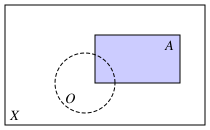
\includegraphics{Subspace_open}}
\caption{A potentially open subset in a subspace.} 
\label{F:Subspace_open}
\end{center}
\end{figure}


\be
\item \label{act:TS_subspace} Show that $\tau_A$ is a topology on $A$.

\vspace{0.1in}

The result of item (1) is that any subset of a topological space $(X,\tau)$ is also a topological space with topology $\tau_A$. 

\begin{definition} \label{def:TS_subspace} Let $(X,\tau)$ be a topological space. A \textbf{subspace}\index{subspace of a topological space} of $(X,\tau)$ is a nonempty subset $A$ of $X$ together with the topology 
\[\tau_A = \{O \cap A \mid O \in \tau\}.\]
\end{definition}

\vspace{0.1in}

\item For each of the following, $X$ is a topological space and $\tau$ is a topology on $X$.
	\ba
	\item Let $X= \{a,b,c,d\}$ and $\tau = \{\emptyset, \{a\}, \{b\}, \{a,b\}, X \}$. Consider the subset $A=\{b,c\}$ and list the open sets in the subspace topology $\tau_A$. Now consider $Z = \{a,b\}$. What is the name of the subspace topology $\tau_Z$ on this subset of $X$?  

	\item  Consider $X=\R$ with $\tau$ the indiscrete topology.  What are the open sets in the subspace topology on $[1,2]$? Now generalize to any nonempty set in the indiscrete topology.

	\item Let $X = \{a,b,c,d,e,f,g,h,i\}$ with $\tau$ the discrete topology. What are the open sets in the subspace topology on $\{a,b,d\}$.  Now generalize to any nonempty set in the discrete topology.

	\item Let $X= \{a,b,c,d,e,f\}$ with $\tau = \{\emptyset,\{a\}, \{c,d\}, \{a,c,d\}, \{b,c,d,e,f\}, X\}$. What are the open sets in the subspace $A = \{a, b, e\}$? Is every open set in $A$ an open set in $X$? Explain.

	\item Let $X=\Z$ with $\tau = \tau_{FC}$ the finite complement topology. What are the open sets in the subspace topology on $A = \{0,19, 37, 5284\}$? Can you generalize this to the subspace topology on any finite subset of $\Z$? 

\item Let $X=\Z$ with $\tau = \tau_{FC}$ the finite complement topology. What are the open sets in the subspace topology on the even integers?  Can you generalize this to the subspace topology on any infinite subset of $\Z$? 

\ea

\ee

\end{pa}


\begin{comment}

\ActivitySolution

\be
\item Since $X \in \tau$ and $X \cap A = A$, we have that $A \in \tau_A$. Also, $\emptyset \in \tau$ and $\emptyset \cap A = \emptyset$. Thus, $\emptyset \in \tau_A$. Now let $U_{\alpha} \in \tau_A$ for all $\alpha$ in some indexing set $I$. For each $\alpha$ there exists $O_{\alpha} \in \tau$ such that $U_{\alpha} = O_{\alpha} \cap A$. Then 
\[\bigcup_{\alpha \in I} U_{\alpha} = \bigcup_{\alpha \in I} A \cap O_{\alpha} = A \cap  \bigcup_{\alpha \in I} O_{\alpha}.\]
But $\bigcup_{\alpha \in I} O_{\alpha} \in \tau$, so it follows that $\bigcup_{\alpha \in I} U_{\alpha} \in \tau_A$. Thus, $\tau_A$ is closed under arbitrary unions. Now let $U_1$, $U_2$, $\ldots$, $U_n$ be in $\tau_A$ for some positive integer $n$. For each $k$ there exists $O_k \in \tau$ such that $U_k = A \cap O_k$. Then
Then 
\[\bigcap_{k=1}^n U_{k} = \bigcap_{k=1}^n A \cap O_{k} = A \cap  \bigcap_{k = 1}^n O_{k}.\]
But $\bigcap_{k=1}^n O_{k} \in \tau$, so it follows that $\bigcap_{k=1}^n U_{k} \in \tau_A$. Thus, $\tau_A$ is closed under finite intersections. We conclude that $\tau_A$ is a topology on $A$. 

\item For each of the following, $X$ is a topological space and $\tau$ is a topology on $X$.
	\ba
	\item  The elements of $\tau_A$ are the intersections of the sets in $\tau$ with $A$. So 
\[\tau_A = \{ \emptyset, \{b\}, A\}.\]
The elements of $\tau_Z$ are the intersections of the sets in $\tau$ with $Z$. So 
\[\tau_Z = \{ \emptyset, \{a\}, \{b\}, \{a,b\}, Z\}.\]
So $\tau_Z$ is the discrete topology on $Z$. 


	\item  The only open sets in the indiscrete topology on a set $X$ are $\emptyset$ and $X$. So if $A$ is a subset of a topological space $X$ with the indiscrete topology, then the induced topology on $A$ is also the indiscrete topology. 


	\item  If $X$ is a topological space with the discrete topology, then every subset of $X$ is open. Thus, if $A$ is a subset of $X$, then $\tau_A = 2^A$. 


	\item  The elements of $\tau_A$ are the intersections of the sets in $\tau$ with $A$. So 
\[\tau_A = \{ \emptyset, \{a\}, \{b,e\}, A\}.\]
The set $\{b,e\}$ is relatively open, but not open in $X$. 

	\item  Recall that the nonempty open sets in $\Z$ are those sets whose complements are finite. Note that the $\Z \setminus \{5\}$ is in $\tau_{FC}$. So if $n \in A$, then $(\Z \setminus \{5\}) \cap \{n\} = \{n\}$. So every subset of $A$ is open and $\tau_{A}$ is the discrete topology. The same argument shows that if $A$ is any finite subset of $\Z$, then the induced topology is the discrete topology. 

\item  Let $\E$ be the set of even integers. We claim that the induced topology is again the finite complement topology. Let $U$ be a subset of $\E$ with $\E \setminus U$ a finite subset of $\E$. Let $O$ be the union of $U$ with the set of odd integers. That is, $O = U \cup (\Z \setminus \E)$. Then $\Z \setminus O = \E \setminus U$ is finite and $O$ is in $\tau_{FC}$. Since $U = \E \cap O$, we have that $U$ is in the subspace topology. Conversely, if $O \in \tau_{FC}$, then $\Z \setminus O$ is finite. Since $\E \subset \Z$, we have $(\E \setminus O) \subseteq (\Z \setminus O)$ and 
\[\E \setminus (\E \cap O) = \E \setminus O\]
 is a finite set. So the only elements in the subspace topology are those whose complements in $\E$ are finite.  
 
 The same argument will show that if $X$ is an infinite topological space with the finite complement topology, then the induced topology on any infinite subset is the finite complement topology. 

\ea

\ee

\end{comment}

\csection{The Subspace Topology}\label{sec_subspace_top}

In our preview activity, we saw that the intersection of the open sets in a topological space $X$ with any nonempty subset $A$ of $X$ forms a topology for $A$. We then have $A$ as a subspace of $X$.  

The topology $\tau_A$ in Definition \ref{def:TS_subspace} is called the \emph{subspace topology}\index{subspace topology}, the \emph{induced topology}\index{induced topology}, or the \emph{relative topology}\index{relative topology}. In our preview activity we saw that sets that are open in a subspace $A$ of a topological space $X$ need not be open in $X$. So we call the sets in $\tau_A$ \emph{relatively open}\index{relatively open set}.  

Once we have defined relatively open sets, we can then consider how to define relatively closed sets. 

\begin{activity} Let $(X, \tau)$ be a topological space, and let $A$ be a subset of $X$.
\ba
\item Recall that a subset of a topological space is closed if its complement is open. Given that $(A, \tau_A)$ is a topological space, how is a closed set in $A$ defined? Such a set will be called \emph{relatively closed}\index{relatively closed set}.

\item Recall that a subset $U$ of $A$ is relatively open if and only if $U = A \cap O$ for some open subset of $X$. With this in mind, how might we expect a relatively closed set in $A$ to be related to a closed set in $X$? State and prove a theorem for this result.  

\ea

\end{activity}

\begin{comment}

\ActivitySolution

\ba
\item A relatively closed set is the complement in $A$ of a relatively open set.

\item
\begin{theorem} Let $(X, \tau)$ be a topological space, and let $A$ be a subset of $X$. A set $C_A \in A$ is relatively closed if and only if $C_A = C \cap A$ for some closed set $C$ in $X$.  
\end{theorem}

\begin{proof} Let $(X, \tau)$ be a topological space, and let $A$ be a subset of $X$. Let $C_A$ be a relatively closed set in $A$. Then $A \setminus C_A$ is a relatively open set in $A$. Thus, $A \setminus C_A = A \cap O$ for some open set $O$ in $X$. Let $C = X \setminus O$. Since $O$ is open in $X$ we know that $C$ is closed in $X$. We will show that $C_A = A \cap C$. Now 
\[C_A = A \setminus (A \setminus C_A) = A \setminus (A \cap O) = A \setminus O = A \cap (X \setminus O) = A \cap C\]
as desired.

For the converse, let $C$ be a closed set in $X$ and suppose $C_A = C \cap A$. To show that $C_A$ is relatively closed, notice that 
\[A \setminus C_A = A \setminus (C \cap A) = A \setminus C = A \cap (X \setminus C).\]
Now $X \setminus C$ is an open set, so $A \setminus C_A$ is a relatively open set. We conclude that $C_A$ is a relatively closed set. 
\end{proof}


\ea

\end{comment}

\csection{Bases for Subspaces}\label{sec_base_sub}

Recall that a basis $\B$ for a topological space is a collection of sets that generate all of the open sets through unions. If we have a basis $\B$ for a topological space $(X, \tau)$, and if $A$ is a subspace of $X$, we might ask if we can find a basis $\B_A$ from $\B$ in a natural way.

\begin{activity} Let $(X, \tau)$ be a topological space with basis $\B$, and let $A$ be a subspace of $X$.
\ba
\item There is a natural candidate to consider as a basis $\B_A$ for $A$. How do you think we should define the elements in $\B_A$?

\item Recall that a set $\B$ is a basis for a topological space $X$ if
\begin{enumerate}
\item For each $x \in X$, there is a set in $\B$ that contains $x$.
\item If $x \in X$ is an element of $B_1 \cap B_2$ for some $B_1, B_2 \in B$, then there is a set $B_3 \in \B$ such that $x \in B_3 \subseteq B_1 \cap B_2$. 
\end{enumerate}
Show that your set from (a) is a basis for the induced topology on $A$.

\ea

\end{activity}

\begin{comment}

\ActivitySolution

\ba
\item It is reasonable to define $\B_A$ as 
\[\B_A = \{B \cap A \mid B \in \B\}.\]

\item Let $a \in A$. Then $a \in X$ so there is a set $B \in \B$ such that $a \in B$. Then $a \in B \cap A$, so $\B_A$ satisfies the first condition of a basis. 

Now suppose $a \in A$ and that $a \in B_1 \cap B_2$ for some $B_1$ and $B_2$ in $\B_A$. By definition of $\B_A$, there are sets $C_1$ and $C_2$ in $\B$ such that $B_1 = A \cap C_1$ and $B_2 = A \cap C_2$. The fact that $\B$ is a basis for $X$ means that there is a set $C_3 \in \B$ such that $a \in C_3 \subseteq C_1 \cap C_2$.   Let $B_3 = A \cap C_3$. Then $a \in B_3$ and 
\[B_3 = A \cap C_3 \subseteq A \cap (C_1 \cap C_2) = (A \cap C_1) \cap (A \cap C_2) = B_1 \cap B_2.\]
It follows that $\B_A$ is a basis for the relative topology on $A$. 

\ea

\end{comment}
 

\csection{Open Intervals and $\R$}\label{sec_open_int_rn}

If we think of a homeomorphism as allowing us to stretch or bend a space, it is reasonable to think that we could stretch an open interval of the form $(a,b)$ infinitely in both directions without altering the nature of the open sets. That is, we should expect that $\R$ with the standard topology is homeomorphic to $(a,b)$ with the subspace topology.   

\begin{activity} Let $a$ and $b$ be real numbers with $a < b$. To show that $(\R, d_E)$ is homeomorphic to $(a,b)$, we need a continuous bijection from $\R$ to $(a,b)$ whose inverse is also continuous. 
\ba
\item First we demonstrate that $(0,1)$ and $\R$ are homeomorphic using the Euclidean metric topology. Let $f : (0,1) \to \R$ be defined by 
\[f(x) = \tan\left(\pi\left(x-\frac{1}{2}\right)\right).\]
	\begin{enumerate}[i.]
	\item Explain why $f$ maps $(0,1)$ to $\R$.
	
	\item Explain why $f$ is an injection.
	
	\item Explain why $f$ is a surjection.
	
	\item Explain why $f$ and $f^{-1}$ are continuous. (Hint: Use a result from calculus.) 
	
	\end{enumerate}

\item The result of (a) is that $\R$ and $(0,1)$ are homeomorphic spaces. To complete the argument that $\R$ is homeomorphic to $(a,b)$, define a function $g: (0,1) \to (a,b)$ and explain why your $g$ is a homeomorphism.

\ea

\end{activity}

\begin{comment}

\ActivitySolution

\ba
\item Let $f(x) = \tan\left(\pi\left(x-\frac{1}{2}\right)\right)$.
	\begin{enumerate}[i.]
	\item Since $\tan(x)$ is defined on $\left(-\frac{\pi}{2}, \frac{\pi}{2}\right)$, we have that $f$ is defined for 
	\[\begin{array}{c}
	-\frac{\pi}{2} < \pi\left(x-\frac{1}{2}\right) < \frac{\pi}{2} \\
	-\frac{1}{2} < x-\frac{1}{2} < \frac{1}{2} \\
	0 < x < 1.
	\end{array}\]
	The output of the tangent function is always a real number, so $f$ maps $(0,1)$ into $\R$. 
	
	\item If $f(a) = f(b)$, then 
	\begin{align*}
	\tan\left(\pi\left(a-\frac{1}{2}\right)\right) &= \tan\left(\pi\left(b-\frac{1}{2}\right)\right) \\
	\tan^{-1}\left(\tan\left(\pi\left(a-\frac{1}{2}\right)\right)\right) &= \tan^{-1}\left(\tan\left(\pi\left(b-\frac{1}{2}\right)\right)\right)  \\
	\pi\left(a-\frac{1}{2}\right) &= \pi\left(b-\frac{1}{2}\right) \\
	a &= b.
	\end{align*}
	Thus, $f$ is an injection. 
	
	\item If $y \in \R$, then 
	\[f\left(\frac{1}{2} + \frac{1}{\pi}\arctan(y)\right) = y,\]
	so $f$ maps $(0,1)$ onto $\R$.
	
	\item Results from calculus apply to $\R$ using the standard metric. Since $f$ is a composite of differentiable functions, we know that $f$ is continuous. Note also that $f$ is invertible with 
	\[f^{-1}(x) = \frac{1}{2} + \frac{1}{\pi}\arctan(x).\]
	We see that $f^{-1}$ is also a differentiable function, therefore continuous. We conclude that $\R$ is homeomorphic to $(0,1)$. 
	 	
	\end{enumerate}

\item Define $g: (0,1) \to (a,b)$ by $g(x) = a+(b-a)x$. As a linear function we know that $g$ is continuous. The fact that $a < b$ implies that $g$ is increasing and invertible. Since $a+(b-a)(0) = a$ and $a+(b-a)(1) = b$, the increasing continuous nature of $g$ shows that $g$ maps $(0,1)$ onto $(a,b)$. The inverse of $g$ is also linear, so $g^{-1}$ is continuous. We conclude that $g$ is a homeomorphism. The transitivity of begin homeomorphic shows that $\R$ is homeomorphic to any open interval of the form $(a,b)$. 

\ea

\end{comment}

It is left to Exercise (\ref{ex:R_intervals}) to show that $\R$ is also homeomorphic to any interval of the form $(a,\infty)$ or $(-\infty,b)$. Later we will determine if $\R$ is homeomorphic to intervals of the form $[a,b)$, $(a,b]$, $[a, \infty)$ or $(-\infty, b]$. 


\csection{Summary}\label{sec_sub_summ}
Important ideas that we discussed in this section include the following.
\begin{itemize}
\item A subspace of a topological space is any nonempty subset of the topological space endowed with the subspace topology. 
\item An open subset in the subspace topology for a subset $A$ of a topological space $X$ is any set of the form $O \cap A$, where $O$ is an open set in $X$. 
\item The relatively open sets are the open sets in a subspace topology. The relatively closed sets are complements of the relatively open sets in a subspace topology. That is, a relatively closed set in the subspace $A$ of a topological space $X$ are the sets of the form $A \cap C$, where $C$ is a closed set in $X$.  
\item The topological space $\R$ with the standard topology is homeomorphic to any open interval as well as open intervals of the form $(a,\infty)$ or $(-\infty,b)$ for any real numbers $a$ and $b$. 
\end{itemize}

\csection{Exercises}\label{sec_sub_exer}

\be


\item Let $X$ and $Y$ be topological spaces and $f: X \to Y$ be a continuous function. If $A$ is a subspace of $X$, prove that $f|_A : A \to Y$ is also continuous.

\begin{comment}

\ExerciseSolution Let $A$ be a subspace of $X$. To show that $f|_A$ is continuous, let $O$ be an open subset of $Y$. Then $f^{-1}(O)$ is open in $X$. So $f^{-1}(O) \cap A$ is open in $A$. We will demonstrate that $f^{-1}(O) \cap A = (f|_A)^{-1}(O)$, which will show that $f|_A$ is continuous. 

Let $x \in f^{-1}(O) \cap A$. Then $x \in f^{-1}(O)$ and $x \in A$. Since $f(x) \in O$ and $x \in A$, it follows that $f|_A(x) \in O$ and $x \in (f|_A)^{-1}(O)$. So $f^{-1}(O) \cap A \subseteq (f|_A)^{-1}(O)$.

Now let $x \in (f|_A)^{-1}(O)$. Then $x$ must be in $A$ and $f|_A(x) \in O$. So $f(x) \in O$ and $x \in f^{-1}(O) \cap A$. We conclude that $(f|_A)^{-1}(O) \subseteq f^{-1}(O) \cap A$ and, consequently, that $f^{-1}(O) \cap A = (f|_A)^{-1}(O)$.

\end{comment}

\item Let $X$ be a topological space, let $A$ be a subspace of $X$, and let $B$ be a subspace of $A$. Show that the subspace topology that $B$ inherits from $A$ is the same as the subspace topology that $B$ inherits from $X$.

\begin{comment}

\ExerciseSolution Let $O$ be an open set in $B$ considered as a subspace of $A$. Then $O = B \cap O_A$ for some set $O_A$ that is open in $A$. Since $O_A$ is open in $A$, there exists an open set $O_X$ in $X$ such that $O_A = A \cap O_X$. But then $O = B \cap O_A = B \cap (A \cap O_X) = B \cap O_X$. So every open set in $B$ as a subspace of $A$ has the form $B \cap O_X$ for some open set $O_X$ in $X$. 

Similarly, if $O_X$ is an open set in $X$, then $A \cap O_X$ is an open set in the subspace $A$. From this it follows that $B \cap (A \cap O_X) = B \cap O_X$ is an open set in $B$ considered as a subspace of $A$. So the subspace topology that $B$ inherits from $A$ is the same as the subspace topology that $B$ inherits from $X$.


\end{comment}

\item Let $A$ be a subspace of a topological space $X$ and let $B$ be a subset of $A$.

\ba

\item Prove that a point $x$ in $A$ is a limit point of $B$ in the subspace topology for $A$ if and only if $x$ is a limit point of $B$ in the topology on $X$.

\item Prove that the closure of $B$ in the subspace topology for $A$ is equal to $\overline{B} \cap A$, where $\overline{B}$ is the closure of $B$ in $X$.

\ea

\begin{comment}

\ExerciseSolution

\ba

\item Suppose $x$ is a limit point of $B$ in the subspace topology for $A$. To show that $x$ is a limit point of $B$ in $X$, let $N$ be a neighborhood of $x$ in $X$. Then $N$ contains an open set $O$ that contains $x$. It follows that $O \cap A$ is a neighborhood of $x$ in $A$. Since $x$ is a limit point of $B$ in $A$, the set $O \cap A$ must contain a point in $B$ different fro $x$. But then $N$ contains a point in $B$ different from $x$ and so $x$ is a limit point of $B$ in $X$.

Conversely, suppose that $x$ is a limit point of $B$ in $X$. To show that $x$ is a limit point of $B$ in $A$, let $N$ be a neighborhood of $x$ in $A$. Then $N$ contains an open set $O$ in $A$ that contains $x$. Since $O$ is open in $A$, there exists an open set $U$ in $X$ such that $O = U \cap A$. But then $U$ is a neighborhood of $x$ in $X$ and so must contain a point in $B$ different from $x$. It follows that $O$ contains a point in $B$ different from $x$, and so does $N$. Therefore, $x$ is a limit point of $B$ in the subspace topology for $A$.

\item The closure of $B$ in $A$ is equal to $B \cup B''$, where $B''$ is the set of limit points of $B$ in $A$, while $\overline{B} = B \cup B'$. So to prove the equality we want, we only need to demonstrate that $B'' = B'$. Part (a) shows exactly this equality. 

\ea

\end{comment}

\item \label{ex:R_intervals} Show that $\R$ is homeomorphic, with the standard topology, to any interval of the form $(a,\infty)$ or $(-\infty,b)$.

\begin{comment}

\ExerciseSolution Let $a \in \R$ and let $f: \R \to (a, \infty)$ be defined by $f(x) = a+e^x$. To show that $f$ is a surjection, let $y \in (a,\infty)$. Then $y = a + z$ for some positive real number $z$. So $f(\ln(z)) = a+e^{\ln(z)} = a+z = a + (y-a) = y$. 

To verify that $f$ is an injection, suppose that $f(x_1) = f(x_2)$ for some real numbers $x_1$ and $x_2$. Then $a+e^{x_1} = a+e^{x_2}$ or $e^{x_1} = e^{x_2}$. Applying the natural log to both sides shows that $x_1 = x_2$. 

Now we need to verify that $f$ and $f^{-1}$ are continuous. Let $(r,s)$ be a basic open set in $\R$. The fact that the exponential function is increasing means that $f((r,s)) = \left(a+e^r, a+e^s\right)$, which is an open set. Thus, $f^{-1}$ is continuous. Now let $(r,s)$ be a basic open set in $(a, \infty)$. Note that $f^{-1}(x) = \ln(x-a)$. The fact that the natural log is increasing shows that $f^{-1}((r,s)) =  (\ln(r-a), \ln(s-a))$ which is an open set. Thus, $f$ is continuous. It follows that $f$ is a homeomorphism and $\R$ is homeomorphic to $(a,\infty)$. 

A similar argument shows that if $b \in \R$, then $g: \R \to (-\infty, b)$ defined by $g(x) = b-e^{x}$ is a homeomorphism. 

\end{comment}

\item Let $X$ be a topological space.
\ba

\item Let $O$ be an open subset of $X$. Prove that a subset $A$ of $O$ is open in $O$ if and only if $A$ is open in $X$. 

\item Let $C$ be a closed subset of $X$. Prove that a subset $B$ of $C$ is closed in $C$ if and only if $B$ is closed in $X$. 

\ea

\begin{comment}

\ExerciseSolution

\ba

\item Let $O$ be an open subset of $X$. Let $A$ be an open subset of $O$. Then there is an open set $U$ in $X$ such that $A = U \cap O$. As the intersection of two open subsets, we conclude that $A$ is open in $X$.

Conversely, let $A$ be a subset of $O$ that is open in $X$. Since $A$ is open in $X$, the set $A \cap O = A$ is open in $A$. 

\item Let $C$ be a closed subset of $X$. Let $B$ be a closed subset of $C$. Then there is a closed set $V$ in $X$ such that $B = V \cap C$. As the intersection of two closed subsets, we conclude that $B$ is closed in $X$.

Conversely, let $B$ be a subset of $C$ that is closed in $X$. Since $B$ is closed in $X$, the set $B \cap C = B$ is closed in $C$. 

\ea

\end{comment}


\item A property of a topological space is said to be hereditary if that property is inherited by every subspace. We state this more  formally in the following definition.

\begin{definition} A property $P$ of a topological space $X$ is \textbf{hereditary}\index{hereditary property} if every subspace of $X$ also has property $P$.
\end{definition}

Show that properties $T_1$, $T_2$, and $T_3$ are hereditary. (The separation axioms $T_i$ are found on page \pageref{sec:Closed_sets_topology}.) The fact that $T_4$ is not hereditary is somewhat difficult. One example is the Tychonoff plank (which is normal) with the Deleted Tychonoff plank (which is not normal) as subspace. An interested reader can consult \emph{Counterexamples in Topology (2nd ed.)}, Lynn Arthur Steen and J. Arthur Seebach, Jr., Dover Publications, 1978.

\begin{comment}

\ExerciseSolution \item Let $X$ be a topological space and $Y$ a subspace of $X$. We consider each property in turn.

	\begin{itemize}
	
	\item Suppose that $X$ is $T_1$. To show that $Y$ is $T_1$, let $y_1$ and $y_2$ be distinct points in $Y$. Then $y_1$ and $y_2$ are distinct points in $X$. The fact that $X$ is $T_1$ implies that there is an open set $O$ in $X$ that contains $y_2$ but not $y_1$. The set $U = O \cap Y$ is open in $Y$ and $y_2 \in U$ but $y_1 \notin U$. We conclude that $Y$ is also $T_1$.
	
	\item This is done in Exercise \ref{ex:Closed_sets:Hausdorff_subspace} on page \pageref{ex:Closed_sets:Hausdorff_subspace}.
	
	\item Suppose that $X$ is $T_3$. Then $X$ is $T_1$ and part (a) shows that $Y$ is $T_1$. So we need to show that $Y$ is regular (this argument also shows that being regular is hereditary). Let $C$ be a closed subset of $Y$ and let $y \in Y \setminus C$. There is a closed subset $D$ of $X$ such that $C = D \cap Y$. Since $y \notin C$ and $y \in Y$, it follows that $y \notin D$. So there exists an open set $O$ in $X$ such that $D \subseteq O$ and $y \notin O$. Let $U = O \cap Y$. Then $U$ is open in $Y$ and 
	\[C = D \cap Y \subseteq O \cap Y = U.\]
Finally, $y \notin O$ so $y \notin U$. We conclude that $Y$ is $T_3$.  
	
	
	\end{itemize}

\end{comment}

\item Suppose that $f : X \to Y$ is a homeomorphism from a topological space $X$ to a topological space $Y$. Let $a \in X$. Must the subspace $X' = X \setminus \{a\}$ of $X$ be homeomorphic to the subspace $Y' = Y \setminus \{f(a)\}$ of $Y$? Prove your conjecture. 

\begin{comment}

\ExerciseSolution The answer is yes. Assume that $f : X \to Y$ is a homeomorphism from a topological space $X$ to a topological space $Y$. Let $a \in X$, and let $X' = X \setminus \{a\}$ and $Y' = Y \setminus \{f(a)\}$. Define $g$ by $g(x) = f(x)$ for all $x \in X'$. Note that the fact that $f$ is an injection shows that $g(x) \neq f(a)$ for any $x \in X'$. Thus, $g : X' \to Y'$. We will prove that $g$ is a homeomorphism, which will imply that $X'$ and $Y'$ are homeomorphic spaces. First we show that $g$ is an injection. 

Let $x_1, x_2 \in X'$ such that $g(x_1) = g(x_2)$. Then $f(x_1) = f(x_2)$. The fact that $f$ is an injection means that $x_1 = x_2$ and so $g$ is an injection. Next we demonstrate that $g$ is a surjection.

Let $y \in Y'$. The fact that $f$ is a surjection implies that there is an $x \in X$ such that $f(x) = y$. Now $y \neq f(a)$, so the fact that $f$ is an injection means that $x \neq a$. Thus, $x \in X'$ and $g$ is a surjection. So $g$ is a bijection from $X'$ to $Y'$. 

Now we need to prove that $g$ and $g^{-1}$ are homeomorphisms. Since $g^{-1}$ is defined by $g^{-1}(y) = f^{-1}(y)$ for all $y \in Y'$, the same argument will work for either $g$ or $g^{-1}$. We demonstrate that $g$ is continuous. Let $O'$ be an open set in $Y'$. Then $O' = O \cap Y'$ for some open set $O$ in $Y$. We know that $f$ is continuous, so $f^{-1}(O)$ is an open set in $X$. Thus, $f^{-1}(O) \cap X'$ is an open set in $X'$. All that remains to do is show that $g^{-1}(O') = f^{-1}(O) \cap X'$. 

Let $x \in g^{-1}(O')$. Then $g(x) \in O' \subseteq O$ and $g(x) \neq f(a)$. Thus, $x \in f^{-1}(O) \cap X'$. Now let $x \in f^{-1}(O) \cap X'$. Then $x \in X'$ and $f(x) = g(x) \in O$. But $x \in X'$ implies $x \neq a$ and so $f(x) = g(x) \in Y'$. So $g(x) \in O \cap Y' = O'$ and so $x \in g^{-1}(O')$. Thus, $g^{-1}(O')$ is an open set in $X$ and $g$ is a continuous function. 

\end{comment}



\item For each of the following, answer true if the statement is always true. If the statement is only sometimes true or never true, answer false and provide a concrete example to illustrate that the statement is false. If a statement is true, explain why. 
	\ba
	\item If $X$ has the discrete topology, then every subspace of $X$ has the discrete topology. 
		
	\item If $X$ is a topological space that does not have the discrete topology, then no subspace of $X$ has the discrete topology.

	\item If $f : X \to Y$ is a continuous function between topological spaces $X$ and $Y$, and $X$ is Hausdorff, then the subspace $f(X)$ of $Y$ is Hausdorff.

	\item If $A$ is a subspace of a topological space $X$ and $B$ is a subset of $X$, then the closure of $B \cap A$ in the subspace topology for $A$ equals $\overline{B} \cap A$, where $\overline{B}$ is the closure of $B$ in $X$. 
	
	\item If $A$ is a subspace of a topological space $X$ and $C$ is a subset of $X$, then the interior of $C \cap A$ in the subspace topology for $A$ equals $\Int(C) \cap A$, where $\Int(C)$ is the interior of $C$ in $X$. 
		
	\ea

\begin{comment}

\ExerciseSolution

\ba

\item This statement is true. Let $A$ be a subset of $X$ and let $B$ be a subset of $A$. Since $A$ is open in $X$, then $A \cap B = B$ is open in $A$. So every subset of $A$ is open and $A$ has the discrete topology. 
		
	\item This statement is false. Let $X = \{a,b,c\}$ with topology $\tau = \{\emptyset, \{a\}, \{b\}, \{a,b\}, X\}$. The subspace topology of the subset $A = \{a,b\}$ of $X$ is the discrete topology. 

\item This statement is false. Let $X = \{a,b,c\}$ with $\tau_X$ the discrete metric, and let $Y = \{a,b,c\}$ with $\tau_Y = \{\emptyset, \{a,b\}, Y\}$. Note that any topological space with the discrete metric is Hausdorff since we can separate points $x$ and $y$ by the open sets $\{x\}$ and $\{y\}$. Let $f : X \to Y$ be the identity map. The inverse image of any open set in $Y$ is open in $X$, so $f$ is continuous. However, $f(X) = Y$ is not Hausdorff because there are no disjoint open sets that separate $a$ and $b$. 

	\item This statement is false. Let $X = \R$ and let $A = \Z$. Let $B$ be the set of irrationals in $X$. Then $A \cap B = \emptyset$ and so the closure of $A \cap B$ in $A$ is empty. Every rational number is a limit of a sequence of irrational numbers, so $\overline{B} = \R$. But this makes $\overline{B} \cap A = A$. 
	
	\item This statement is false. Let $X = \R$ and let $A = \Z$. Let $B$ be the set of rationals in $X$. Then $A \cap B = A$. The subspace topology on $A$ is the discrete topology, so the interior of $A \cap B$ in $A$ is $A$. Every open interval that contains a rational number also contains an irrational number. So $\Int(B) = \emptyset$. But this makes $\Int(B) \cap A = \emptyset$. 	
	
\ea


\end{comment}

\ee
